%!TEX TS-program = xelatex

\documentclass[t]{beamer}

\usetheme{Hannover}
\usecolortheme{rose}

\usepackage{fontspec,xltxtra,xunicode}      %% подготавливает загрузку шрифтов Open Type, True Type и др.
%\defaultfontfeatures{Ligatures={TeX},Renderer=Basic}  %% свойства шрифтов по умолчанию
\setmainfont[Ligatures={TeX,Historic},
SmallCapsFont={Brill},
SmallCapsFeatures={Letters=SmallCaps}]{Brill} %% задаёт основной шрифт документа
\setsansfont{Brill}                    %% задаёт шрифт без засечек
\setmonofont[Ligatures=NoCommon]{DejaVu Sans}
\newfontfamily\SYM{Brill}
\usepackage{indentfirst}
%%% Дополнительная работа с математикой
\usepackage{amsmath,amsfonts,amssymb,amsthm,mathtools} % AMS
\usepackage{icomma} % "Умная" запятая: $0,2$ --- число, $0, 2$ --- перечисление

%%% Работа с картинками
\usepackage{wrapfig} % Обтекание рисунков текстом
\usepackage{rotating}
\usepackage{fixltx2e}
\usepackage{hhline}
\usepackage{lscape}

%%% Работа с таблицами
\usepackage{array,tabularx,tabulary,booktabs} % Дополнительная работа с таблицами
\usepackage{longtable}  % Длинные таблицы
\usepackage{multirow} % Слияние строк в таблице

\usepackage{multicol} % Несколько колонок
%%% Страница
%\usepackage{fancyhdr} % Колонтитулы
% 	\pagestyle{fancy}
 	%\renewcommand{\headrulewidth}{0pt}  % Толщина линейки, отчеркивающей верхний колонтитул
% 	\lfoot{Нижний левый}
% 	\rfoot{Нижний правый}
% 	\rhead{Верхний правый}
% 	\chead{Верхний в центре}
% 	\lhead{Верхний левый}
%	\cfoot{Нижний в центре} % По умолчанию здесь номер страницы

\usepackage{setspace} % Интерлиньяж
%\onehalfspacing % Интерлиньяж 1.5
%\doublespacing % Интерлиньяж 2
\singlespacing % Интерлиньяж 1

\usepackage{subfig} % подкартинки
\usepackage{lastpage} % Узнать, сколько всего страниц в документе.
\usepackage{soul} % Модификаторы начертания
\usepackage{bbding}
\usepackage{tikz} % Работа с графикой
\usepackage{pgfplots}
\usepackage{pgfplotstable}
\usepackage{verbatim}

\usepackage{attachfile2}
\usepackage{alltt}

%%% Лингвистические пакеты
%\usepackage{savetrees} % пакет, который экономит место
\usepackage{forest} % для рисования деревьев
\usepackage{vowel} % для рисования трапеций гласных
\usepackage{natbib}
\bibpunct[: ]{[}{]}{;}{a}{}{,}
\usepackage[nogroupskip,nopostdot, nonumberlist]{glossaries}
%\usepackage{glossary-mcols} 
%\setglossarystyle{mcolindex}
\usepackage{philex} % пакет для примеров
\newcommand{\mytem}{\item[$\circ$]}
\addto\captionsrussian{
\renewcommand{\refname}{}}

\newcommand{\apostrophe}{\XeTeXglyph\XeTeXcharglyph"0027\relax}
\usetikzlibrary{patterns}

\usepackage{ulem}

\usepackage{hyperref}
\setbeamercolor{alerted text}{fg=blue}
\setbeamersize{text margin left=4mm,text margin right=1mm} 
\setbeamertemplate{frametitle}[default][center]
\setbeamertemplate{navigation symbols}{
	\usebeamerfont{footline}%
    \usebeamercolor[fg]{footline}%
    \hspace{1em}%
    {{\small презентация доступна: \href{https://goo.gl/Rtu5Br}{\textbf{https://goo.gl/Rtu5Br}}}
    \hspace{4cm}
    \insertframenumber/\inserttotalframenumber\vspace{0.5mm}}}
\title[]{Introduction to Acoustic Phonetics}
\author[]{G. Moroz}
\date{3 February, 2018}
\begin{document}
\frame{\titlepage}
\section{course}
\begin{frame}{About course}
\begin{itemize}
\item \href{https://agricolamz.github.io/m_Instrumental_Phonetics_2016-2017/}{Here} is a course website.
\item \href{https://www.hse.ru/data/2016/09/19/1117088299/program-1542588518-dLqdKf3_0G.pdf}{Here} is a course program.
\item We expect some theoretical knowledge
\begin{itemize}
\item read 2. chapter from \citep{gussenhoven11}
\item be able to use IPA symbols
\end{itemize}
\item We expect some basic R skills:
\begin{itemize}
\item import .csv files to R
\item dplyr, ggplot2
\end{itemize}
\end{itemize}
\end{frame}
\section{Phonetics}
\begin{frame}{Phonetics?...}
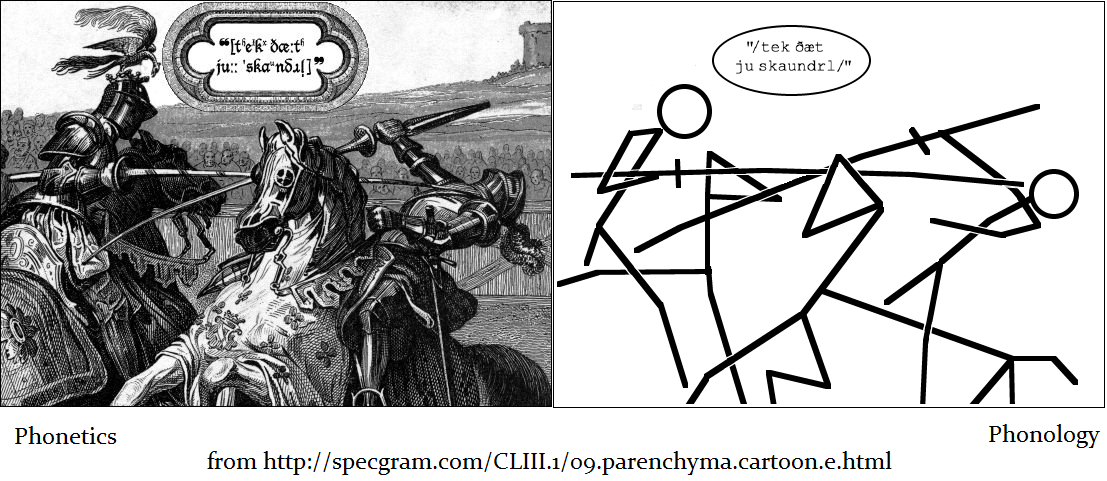
\includegraphics[width=\linewidth]{03-Phonetics-vs-Phonology.png}\\
Phonetics is generally assumed to be a subfield that deals with \textbf{articulatory}, \textbf{acoustic} and \textbf{perceptional} aspects of phonological units. Phonology and phonetics together are supposed to describe organization of sounds in languages. \bigskip\\
This course is about \textbf{acoustic  phonetics}.

\end{frame}
\section{SHM}
\begin{frame}{Simple Harmonic Motion}
\textbf{Periodic Motion} is any type of motion that repeats itself after successuve equal time intervals. \medskip\\
\textbf{Simple Harmonic Motion} is specific type of periodic motion that arises from
\begin{itemize}
\item existence of some \textbf{equilibrium position} for a described object;
\item \textbf{linear restoring force} that tending to pull the described object back to its equilibrium position.
\end{itemize}
\vfill
\begin{center}
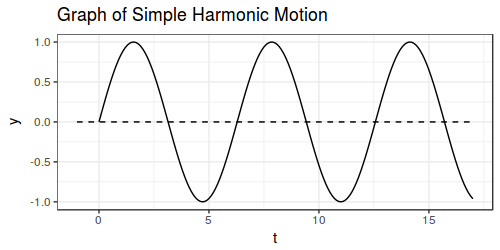
\includegraphics[width=0.7\linewidth]{04-SHM.png}
\end{center}
\end{frame}
\begin{frame}{Simple Harmonic Motion}
\textbf{Amplitude} is the maximum displacement of the equilibrium position.\medskip\\
\textbf{Period (T)} is the duration of time of one cycle in a repeating event.\hfill (s)\medskip\\
\textbf{Frequency (f)} is the number of period (cycles) per second. \hfill (Hz)\bigskip\\
\hfill $ f = \frac{1}{T}$ \hfill $T = \frac{1}{f} $\hfill ${}$\\
\vfill
\begin{center}
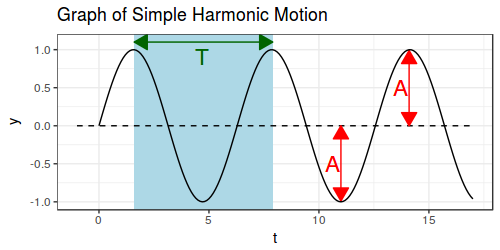
\includegraphics[width=0.7\linewidth]{05-SHM-annotated.png}
\end{center}
\nocite{berg05}
\end{frame}

\section{Sound}
\begin{frame}{Sound as SHM}
We can correlate the physical properties of sound waves with our perception:
\begin{itemize}
\item We perceive changes in frequency as \textbf{pitch}
\item We perceive changes in amplitude as \textbf{loudness}
\end{itemize}
\end{frame}

\section{Phase}
\begin{frame}{Phase of SHM}
One period of SHM can be devided into 360$^{0}$ of \textbf{phase φ}.\medskip\\
\vfill
\begin{center}
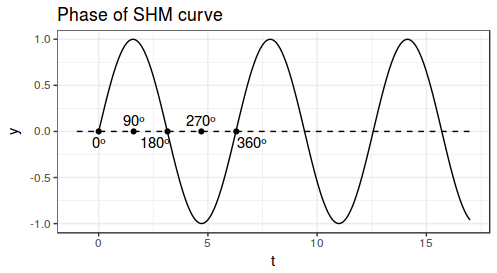
\includegraphics[width=0.7\linewidth]{06-Phase.png}
\end{center}
\end{frame}

\begin{frame}{SHMs comparison}
\begin{center}
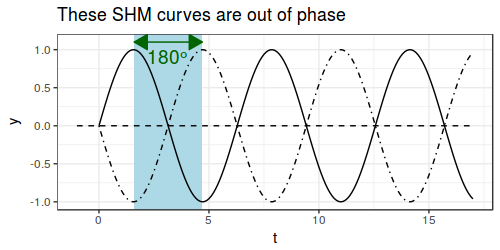
\includegraphics[width=0.7\linewidth]{07-Out-of-Phase.png}
\end{center}
\begin{center}
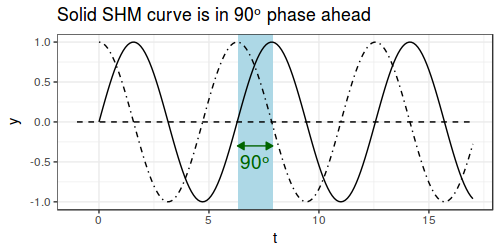
\includegraphics[width=0.7\linewidth]{08-Phase-Ahead.png}
\end{center}
\end{frame}

\begin{frame}{Wave representation}
Waves can be represented by formula:
$$s(t) = A \times \cos(2\pi ft+\phi)$$
\begin{itemize}
\item $A$ --- amplitude
\item $f$ --- is the fundamental frequency
\item $\phi$ --- phase
\item $t$ --- time
\end{itemize}
\end{frame}

\section{Harmonic motion}
\begin{frame}{Harmonic motion}
\begin{center}
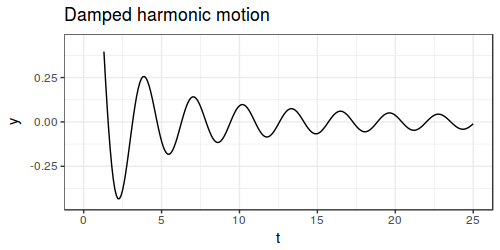
\includegraphics[width=0.7\linewidth]{09-Damped-hm.png}
\end{center}
\begin{center}
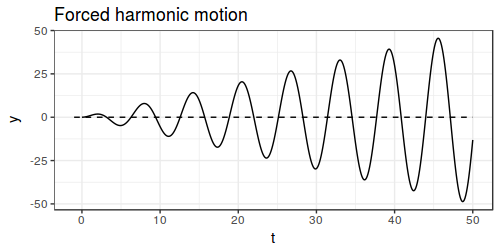
\includegraphics[width=0.7\linewidth]{10-Forced-hm.png}
\end{center}
\end{frame}

\begin{frame}{Harmonic motion}
Harmonic motions are closely related with the phenomena of \textbf{resonance} and \textbf{antiresonance}. \medskip\\
\textbf{Resonance} is a phenomenon in which a vibrating system or external force drives another system to oscillate with greater amplitude at specific frequencies.\medskip\\
\textbf{Antiresonance} is a phenomenon in which a vibrating system or external force drives another system to oscillate with smaller amplitude at specific frequencies.
\end{frame}

\section{Addition of waves}
\begin{frame}{Addition of waves}
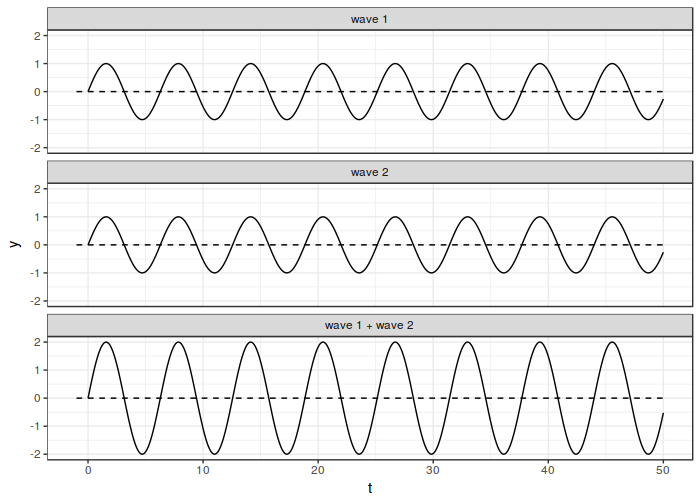
\includegraphics[width=0.9\linewidth]{11-wave-addition.png}
\end{frame}

\begin{frame}{Addition of waves}
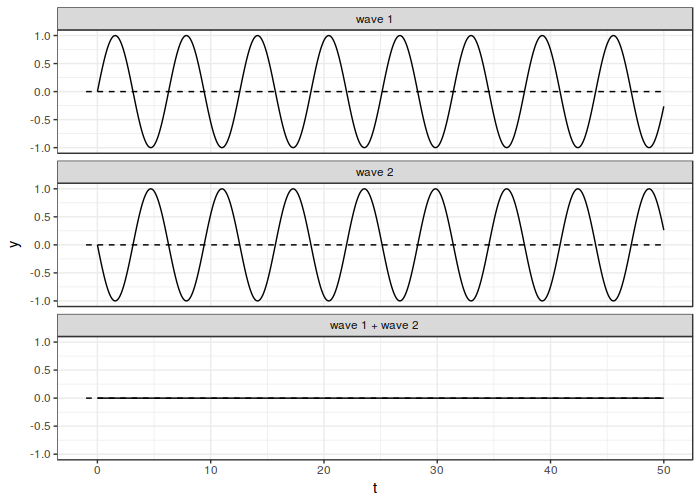
\includegraphics[width=0.9\linewidth]{12-wave-addition.png}
\end{frame}

\begin{frame}{Addition of waves}
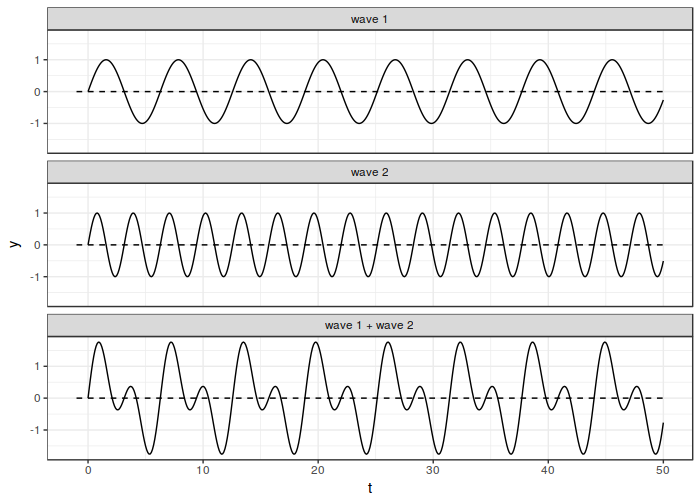
\includegraphics[width=0.9\linewidth]{13-wave-addition.png}
\end{frame}

\begin{frame}{Addition of waves}
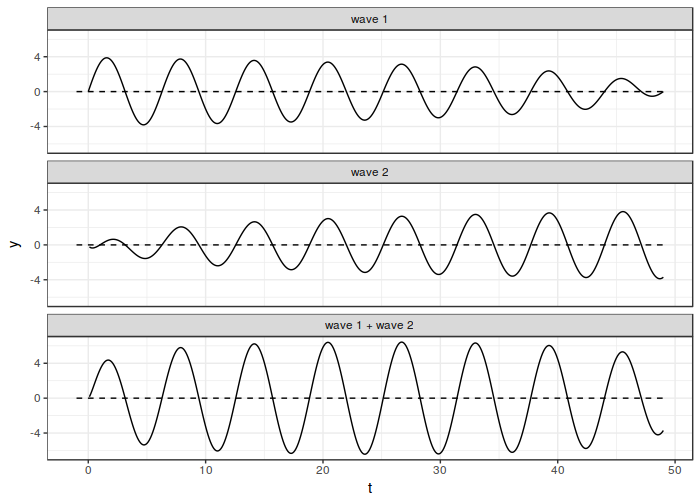
\includegraphics[width=0.9\linewidth]{14-wave-addition.png}
\end{frame}

\begin{frame}{Beats}
\textbf{Beats} is a phenomenon of the change in amplitude of the sum of two waves with slightly different frequencies.
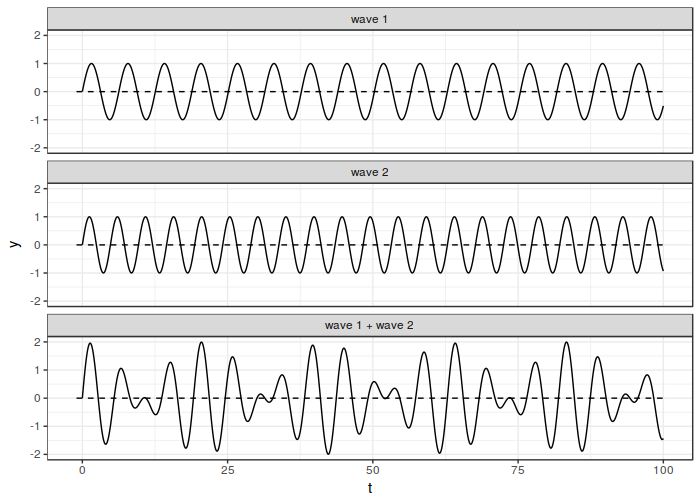
\includegraphics[width=0.9\linewidth]{15-beats.png}
\end{frame}

\section{Spectrogram}
\begin{frame}
\textbf{Fourier Transform} allows to extract components of the complex wave. \vfill
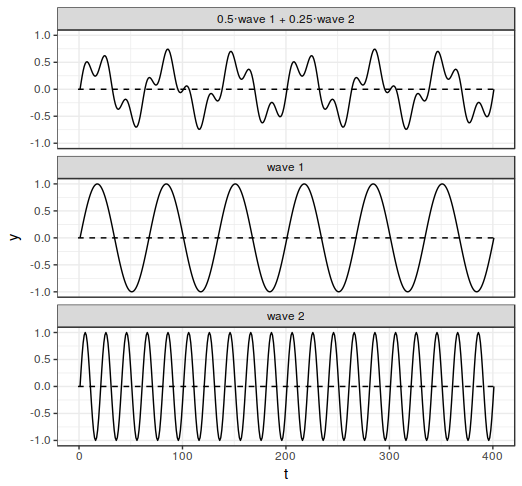
\includegraphics[width=0.8\linewidth]{16-complex.png}
\end{frame}

\begin{frame}
\textbf{Fourier Transform} allows to extract components of the complex wave. \vfill
\begin{tabular}{lll}

\multicolumn{1}{c}{smoothie} &  & \multicolumn{1}{c}{complex wave} \\ 
\multicolumn{1}{c}{↓} & \multicolumn{1}{c}{} & \multicolumn{1}{c}{↓} \\ 
1 banana, cut in chunks &  & 300 Hz \\ 

1 cup grapes  &  & 1000 Hz \\ 
vanilla yogurt &  & \\ 
1/2 apple, cored and chopped &  &  \\ 
1.5 cup fresh spinach leaves  &  &  \\ 
\end{tabular}
\end{frame}

\begin{frame}{Spectrogram}
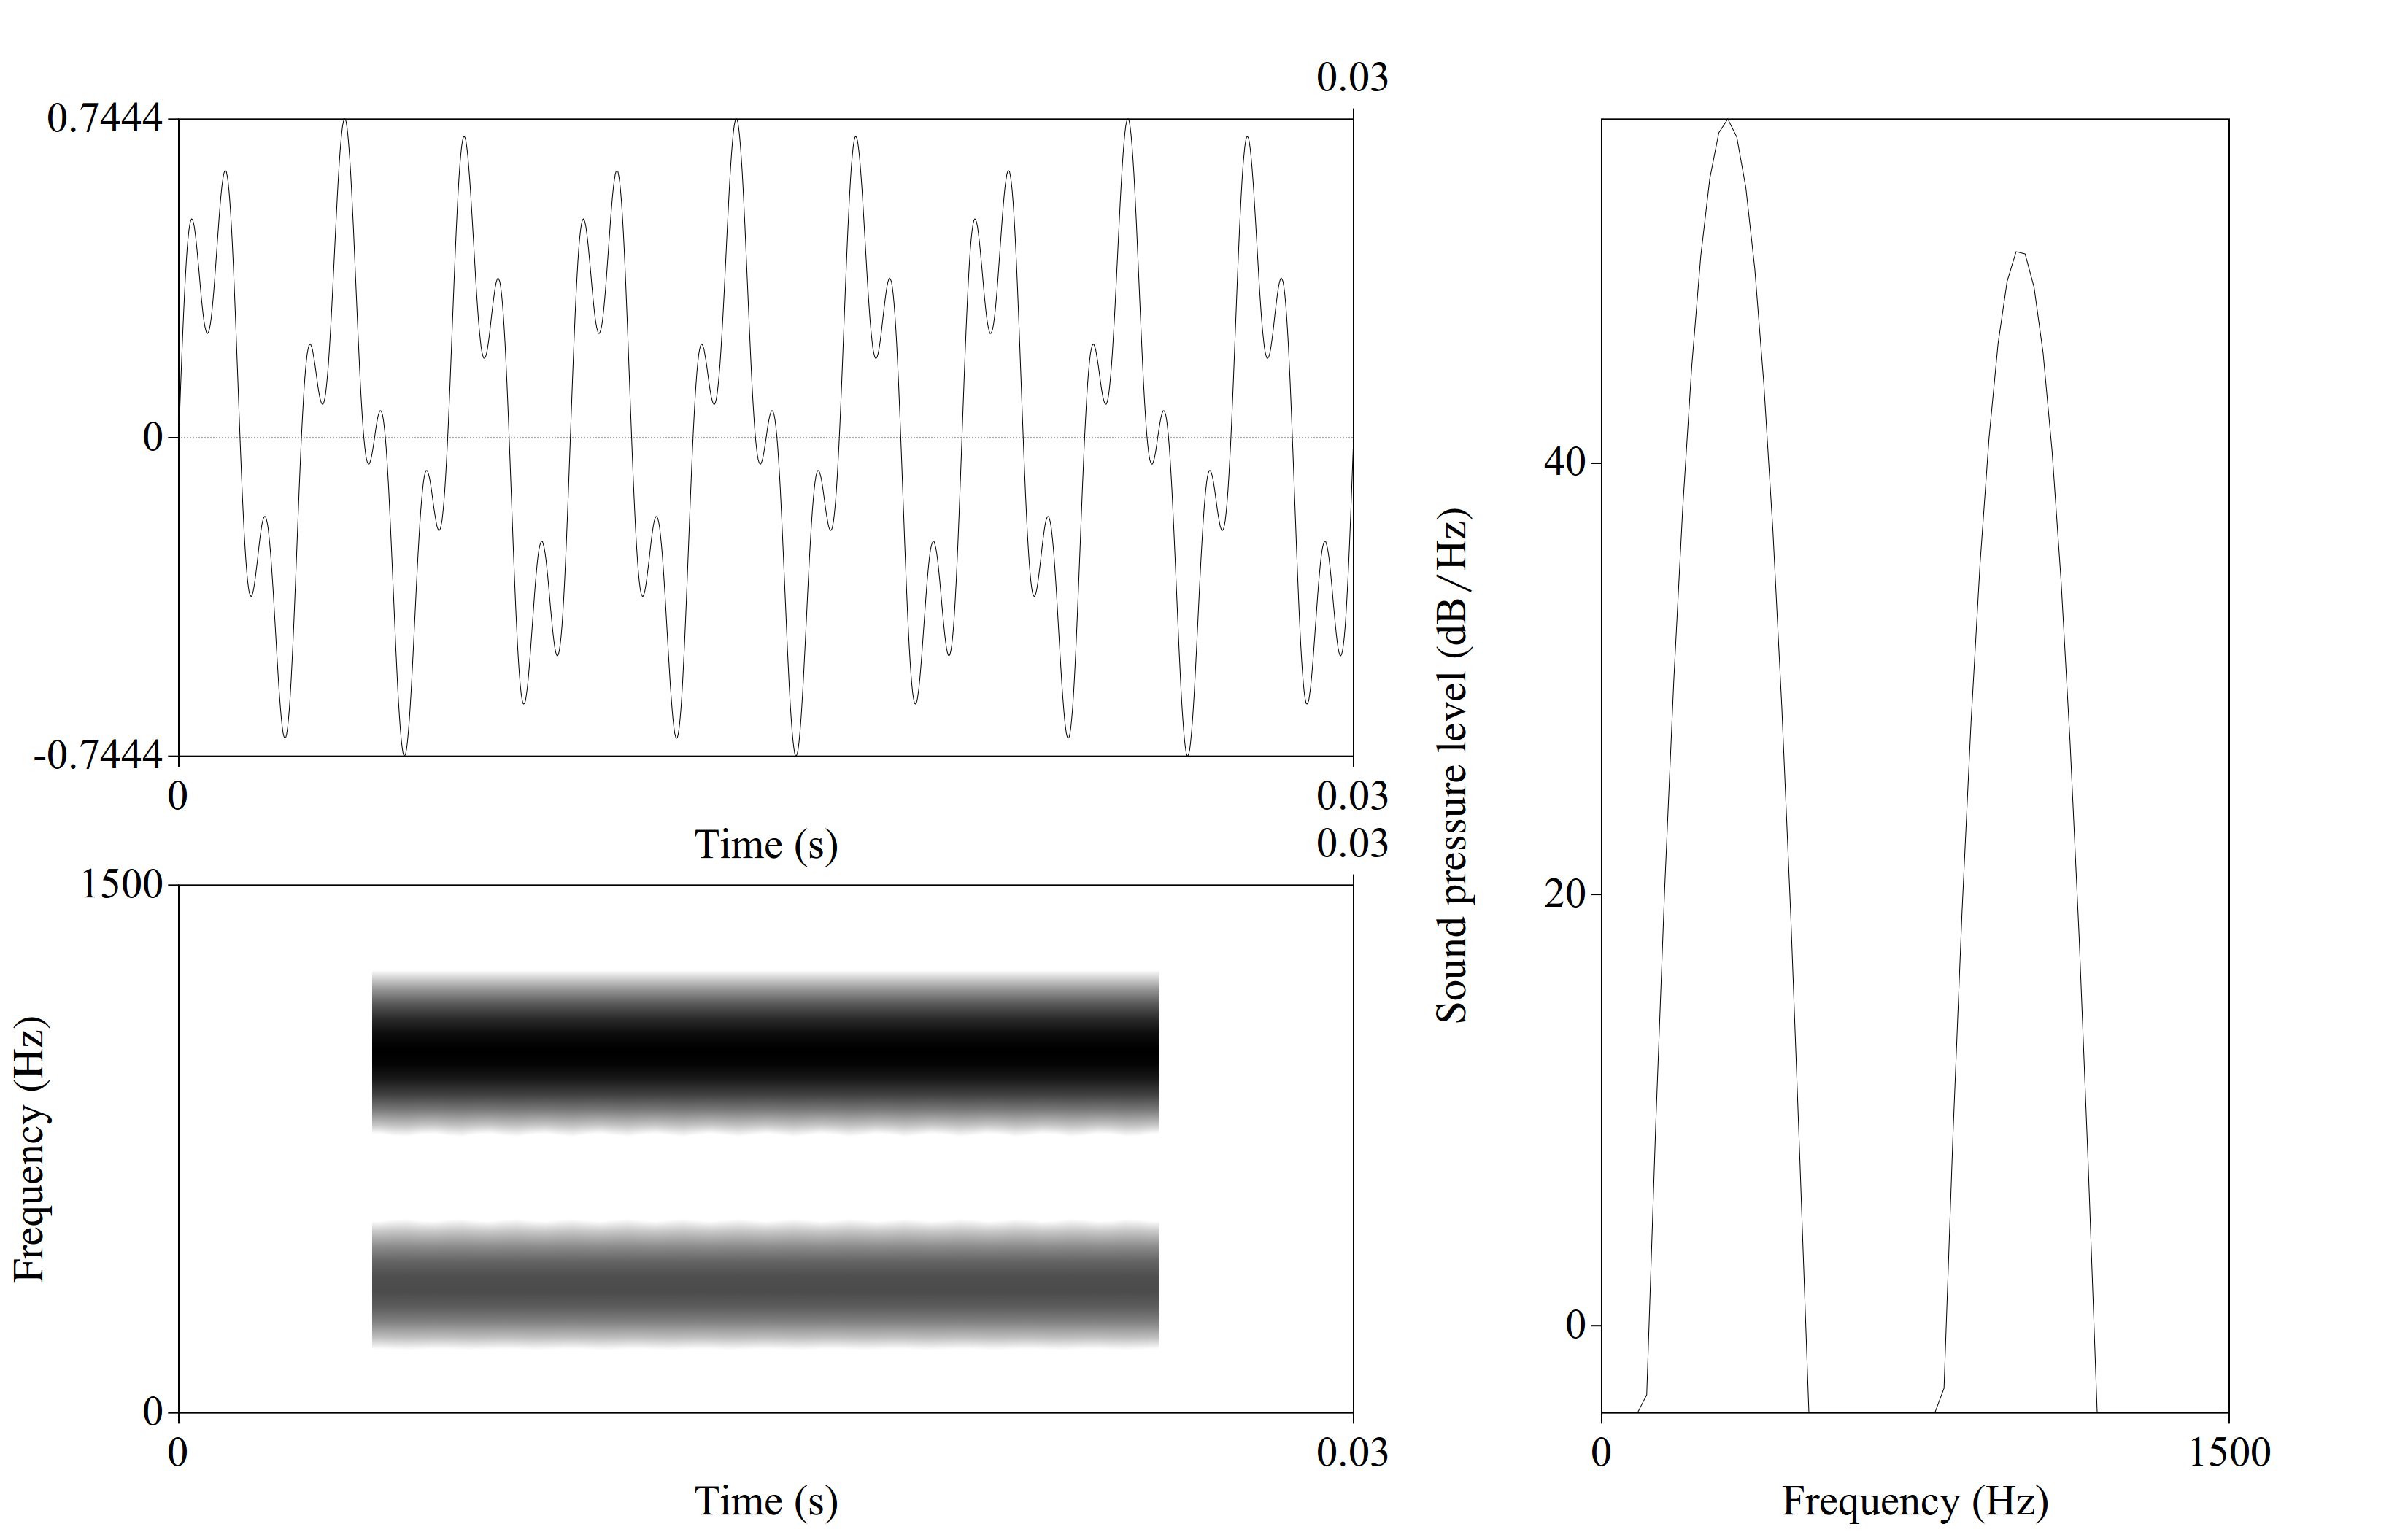
\includegraphics[width=\linewidth]{17-fourier-spectrum.png}
\end{frame}

\begin{frame}{Spectral slices}
Spectrograms are differ in window length
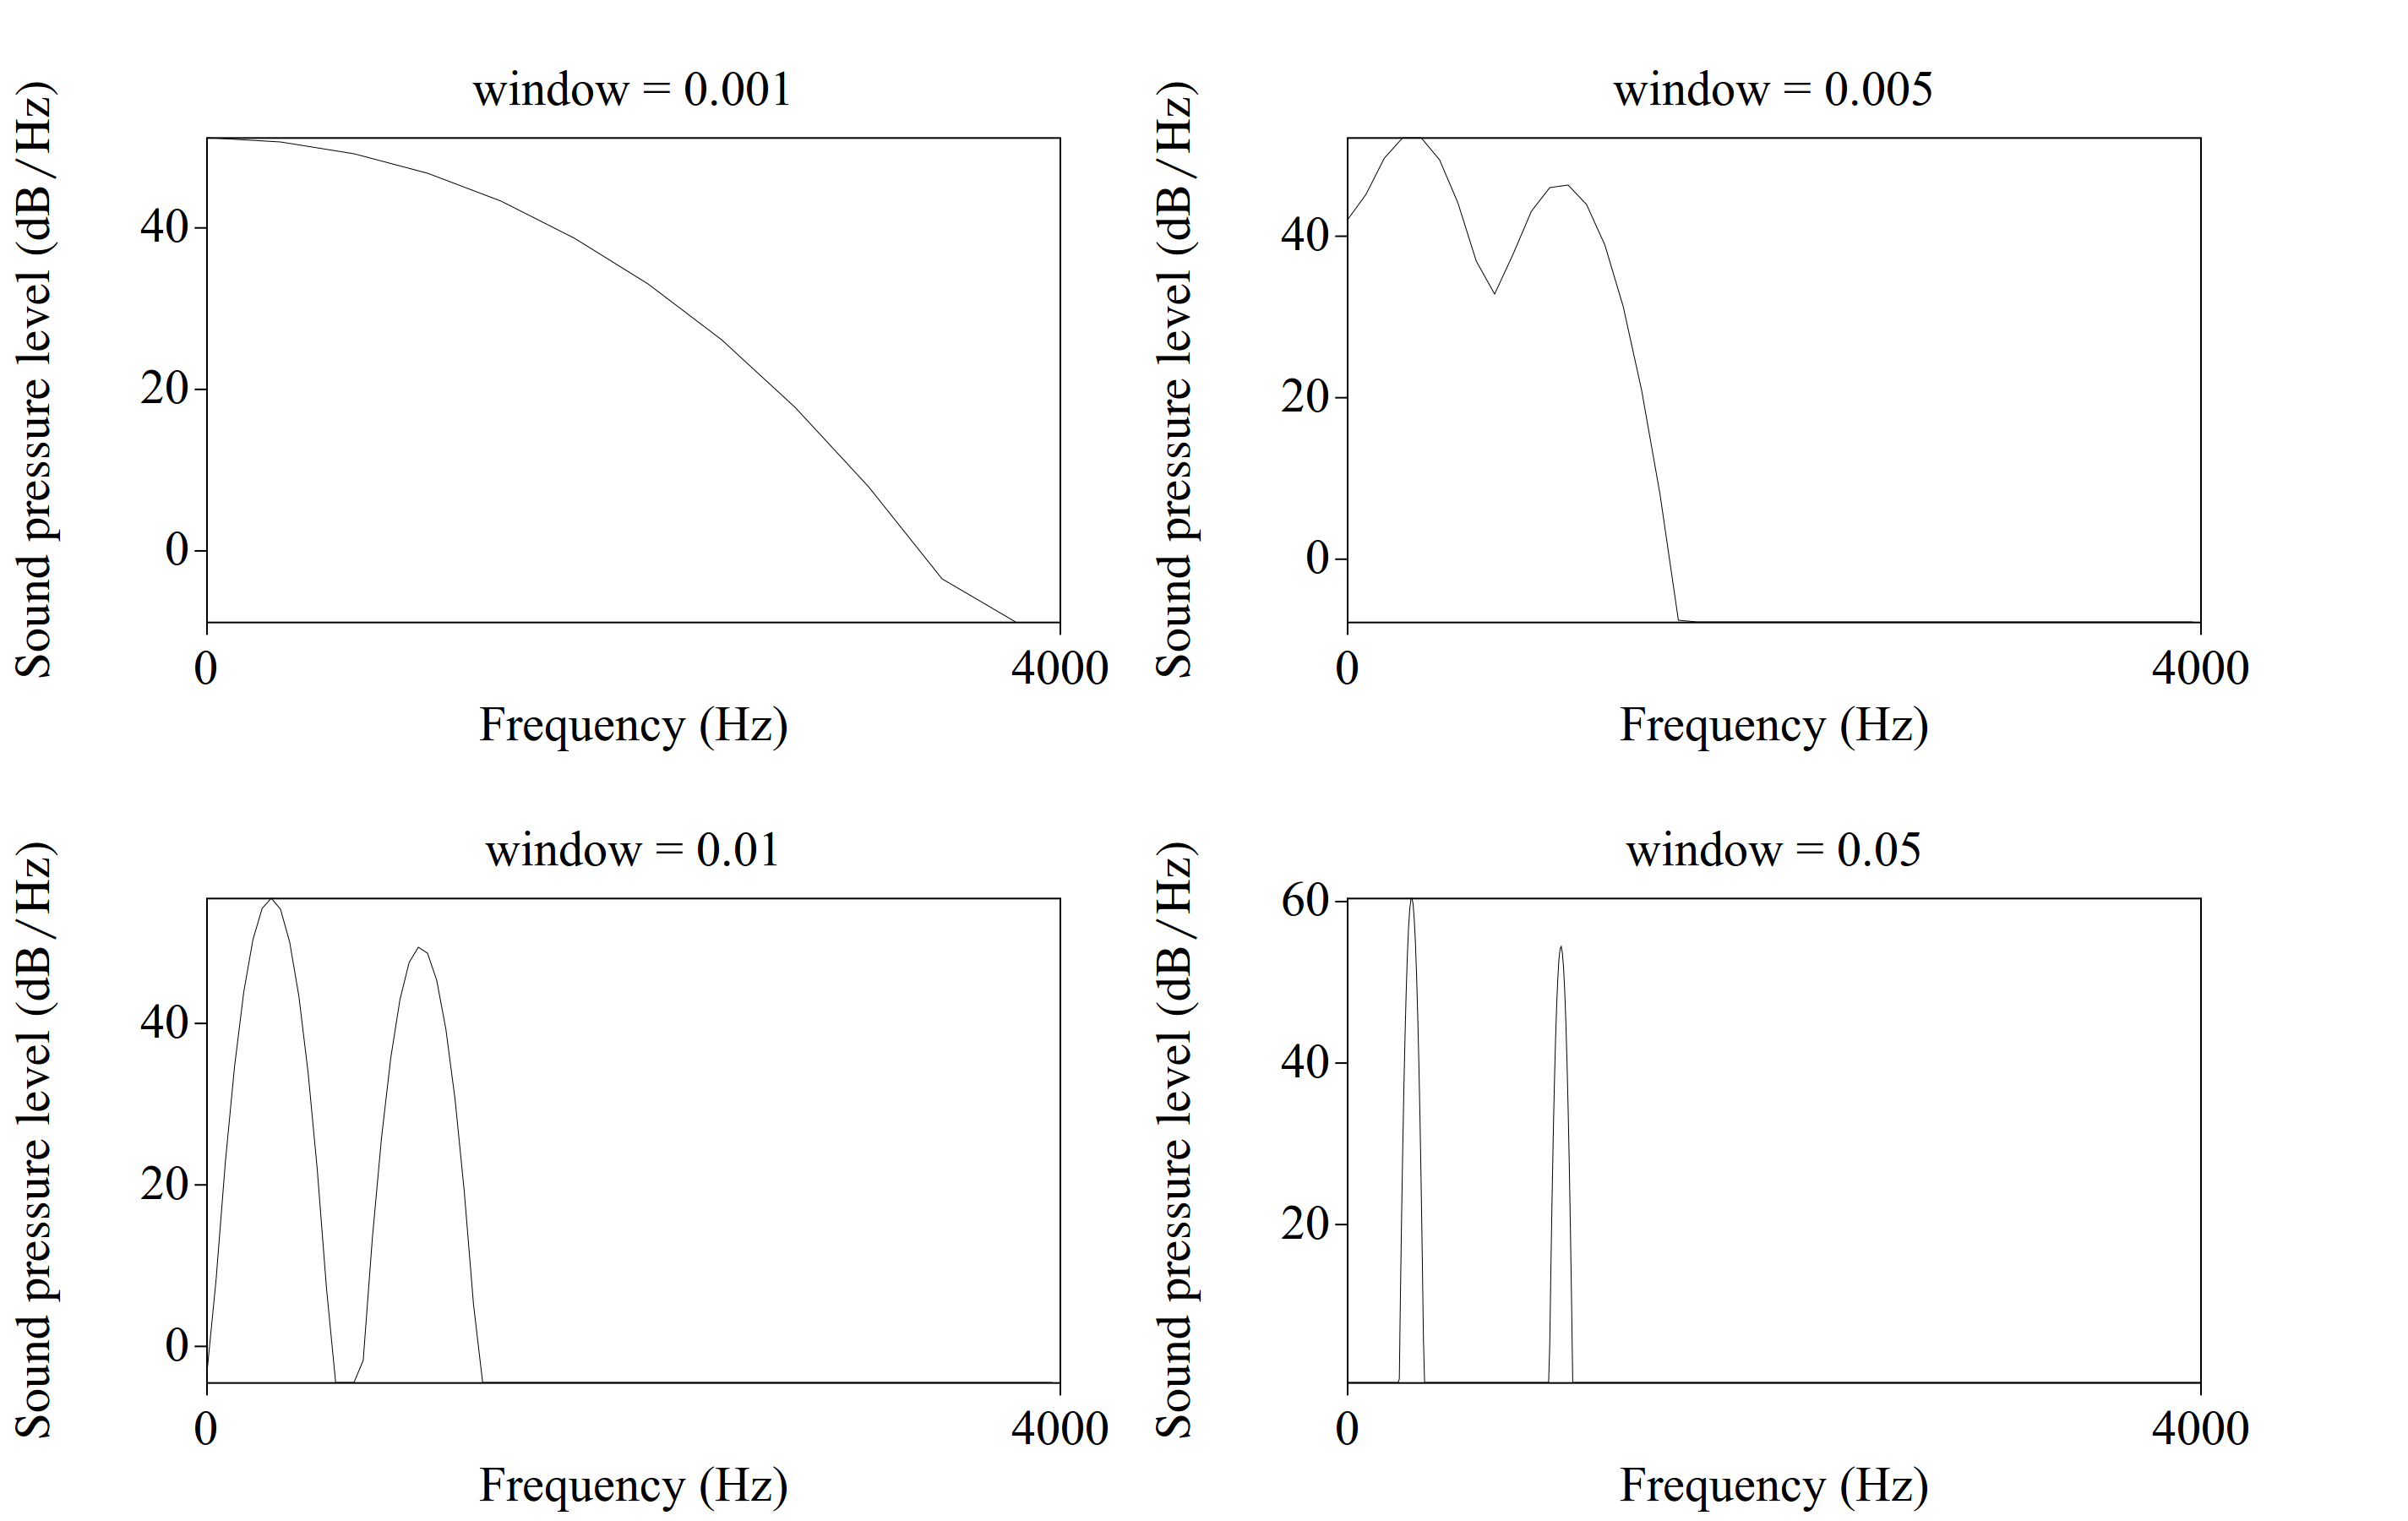
\includegraphics[width=\linewidth]{18-fourier-spectrum.png}
\end{frame}

\begin{frame}{Spectrograms}
Syllable [ka]
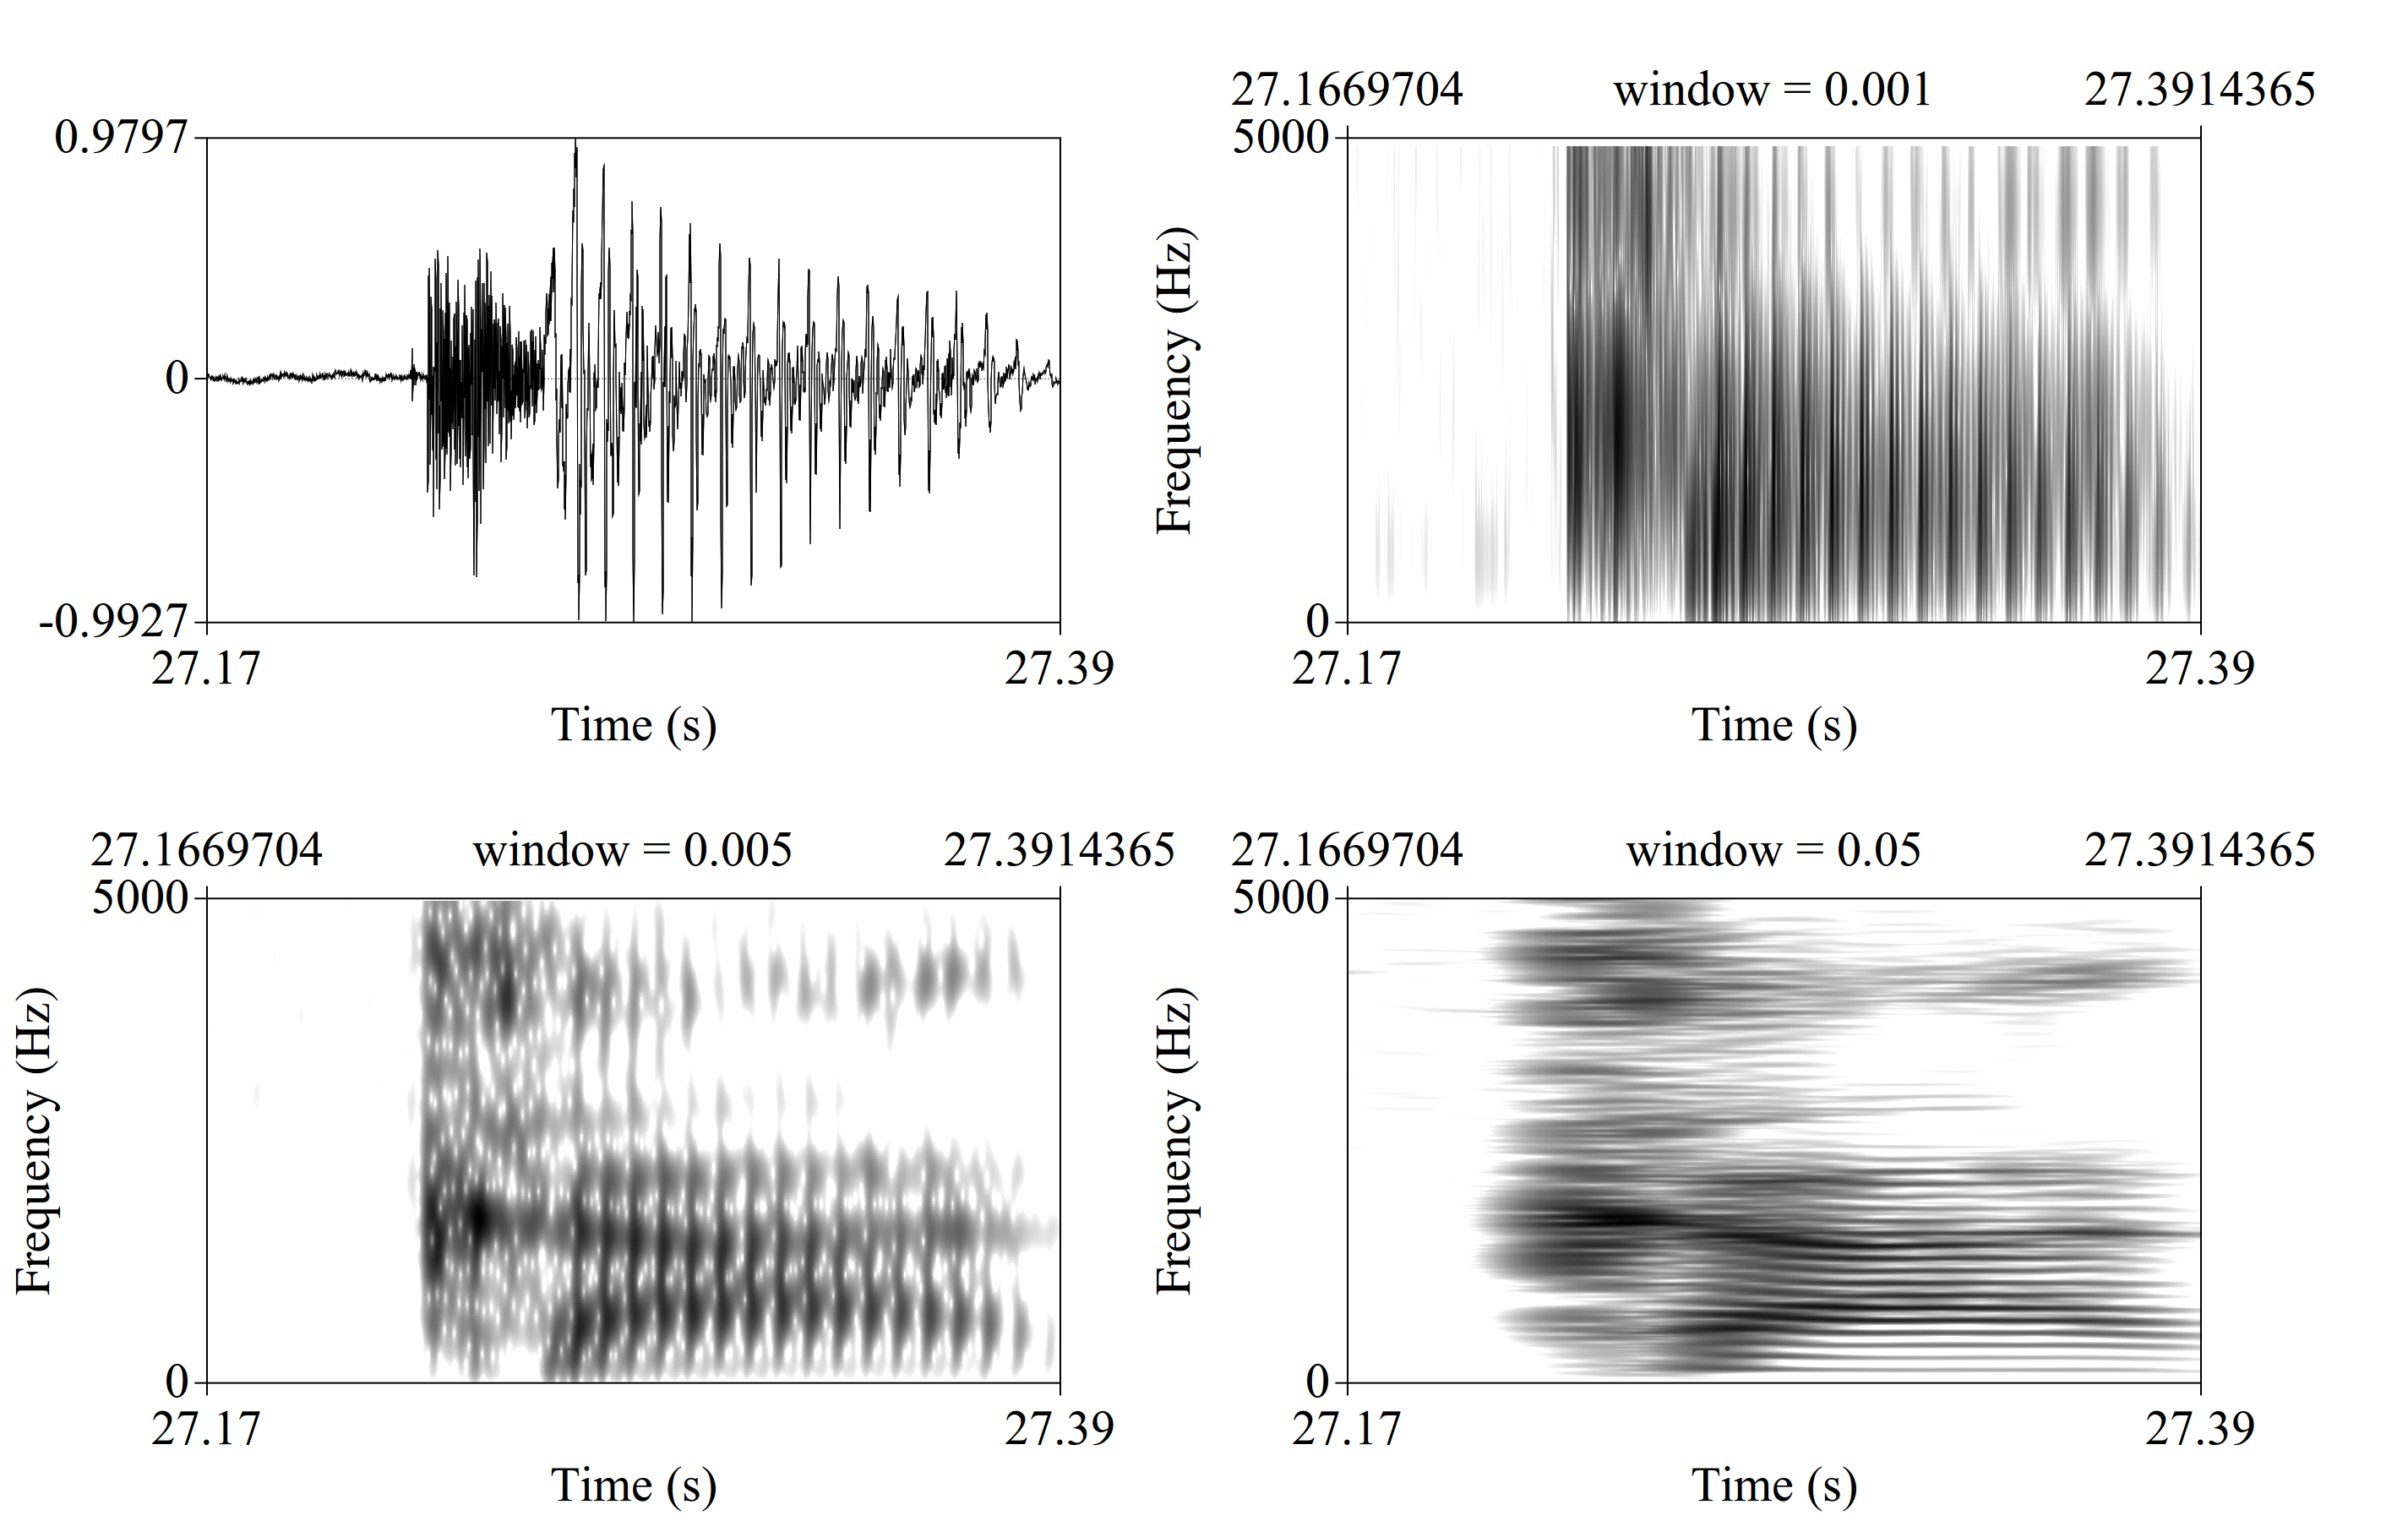
\includegraphics[width=\linewidth]{19-fourier-spectrum.png}
\end{frame}

\begin{frame}{Not by Fourier alone}
Conventional spectrogram and Zhao-Atlas-Marks distribution of the English word \textit{had}, computed using a Kaiser tapering function.
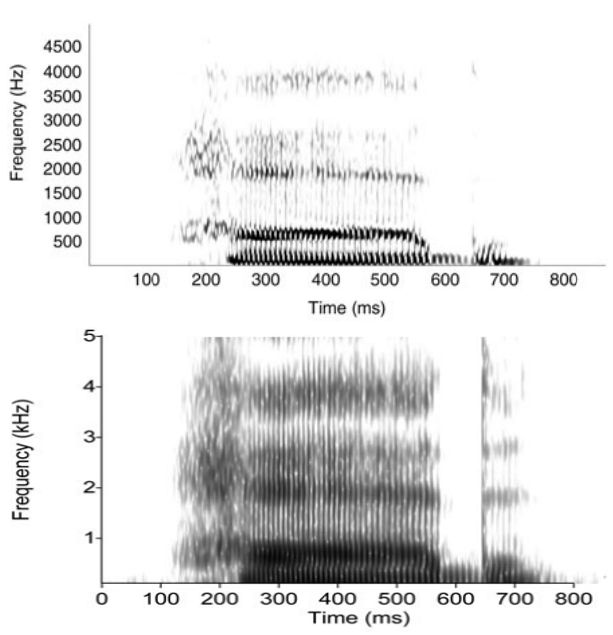
\includegraphics[width=0.63\linewidth]{20-ZAM} from \cite[119]{fulop11}
\end{frame}


\begin{frame}{Not by Fourier alone}
Conventional and reassigned spectrograms of the English word \textit{right}
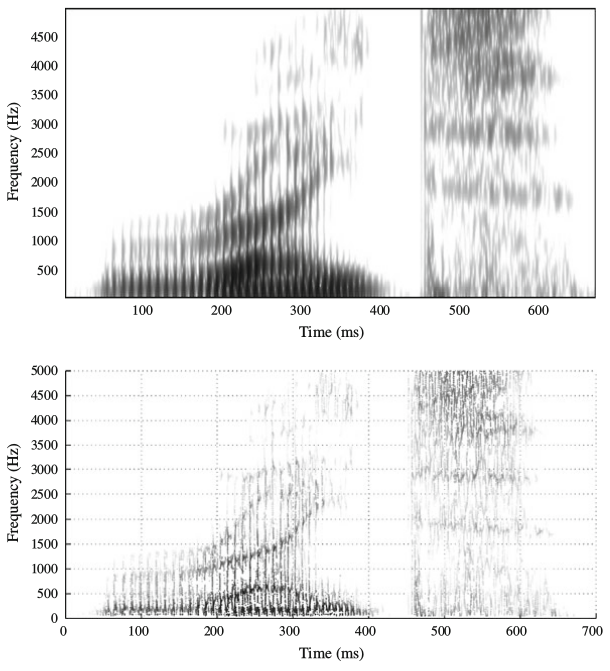
\includegraphics[width=0.63\linewidth]{21-reassigned-spectrum} from \cite[142]{fulop11}
\end{frame}

\section{Source-Filter Model}
\begin{frame}{Source-Filter Model of Speech Production}
The output energy (at the mouth) for a given frequency is equal to the amplitude the source harmonic, multiplied by the magnitude of the filter function for that the frequency.
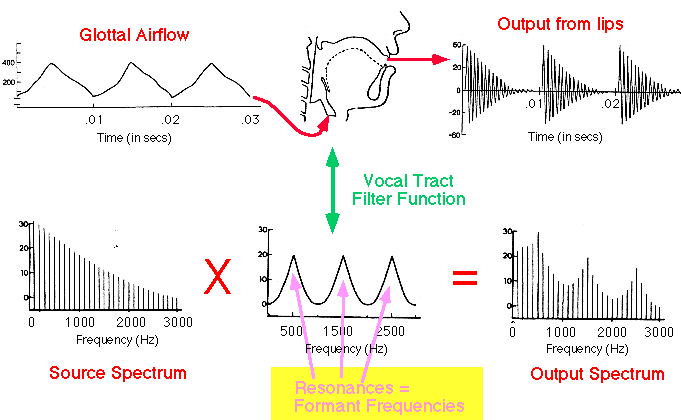
\includegraphics[width=0.95\linewidth]{22-source-filter.png}
\end{frame}

\section{Summary}
\begin{frame}{Summary}
\begin{itemize}
\item sounds are waves (with amplitude, frequency and phase)
\item simple waves can be combined to the complex one
\item Fourier transform allows to extract components of the complex wave
\item It is not only Fourier transform that allows to extract components of the complex wave
\item Source-Filter Model: vocal tract is a resonator that filters some frequencies of the wave produced by vocal folds vibration.
\end{itemize}
\end{frame}
\section{}

\begin{frame}
{\huge Thank you!\bigskip\\
\normalsize Please, don't hesitate to write me\\
agricolamz@gmail.com
\vspace{-130pt}}
\end{frame}
\begin{frame}{Reference}
\footnotesize
\bibliographystyle{chicago}
\bibliography{bibliography}
\end{frame}
\end{document}
